\subsection{TOPOLOGICAL GROUPS}

In the first four sections of this chapter the law of composition of a group will generally be written multiplicatively, and e shall denote the identity element; translation of results into additive notation (which, we recall, is reserved exclusively to commutative groups) is usually left to the reader.

DEFINITION 1. A topological group is a set G which carries a group structure and a topology and satisfies the following two axioms:

\((\mathrm{GT}_{\mathbf{I}})\) . The mapping \((x, y) \to xy\) of \(\mathbf{G} \times \mathbf{G}\) into \(\mathbf{G}\) is continuous.

\((\mathbf{G}\mathbf{T}_{\mathbf{II}})\) . The mapping \(x \to x^{-1}\) of \(\mathbf{G}\) into \(\mathbf{G}\) (the symmetry of the group \(\mathbf{G}\) ) is continuous.

A group structure and a topology on a set G are said to be compatible if they satisfy \((\mathrm{GT}_{\mathbf{I}})\) and \((\mathrm{GT}_{\mathbf{II}})\) .

Examples. 1) The discrete topology on a group G is compatible with the group structure. A topological group whose topology is discrete is called a discrete group.

Again, the coarsest topology (Chapter I, § 2, no. 2) on G is compatible with the group structure of G.

* 2) In Chapter IV we shall see that the topology of the rational line Q (resp. the real line R) is compatible with the additive group structure of Q (resp. R). *

\begin{enumerate}
\def\labelenumi{\arabic{enumi})}
\setcounter{enumi}{2}
\tightlist
\item
  If G is a topological group, its topology is compatible with the structure of the group \(G^{0}\) which is the opposite of G; \(G^{0}\) , with this topology, is said to be the topological group opposite to G.
\end{enumerate}

Axioms \((\mathrm{GT}_{\mathrm{I}})\) and \((\mathrm{GT}_{\mathrm{II}})\) are equivalent to the following :

\((\mathbf{GT}^{\prime})\) . The mapping \((x,y)\to xy^{-1}\) of \(\mathbf{G}\times \mathbf{G}\) into \(\mathbf{G}\) is continuous.

Clearly \((\mathrm{GT}_{\mathbf{I}})\) and \((\mathrm{GT}_{\mathbf{II}})\) together imply \((\mathrm{GT}^{\prime})\) . Conversely, \((\mathrm{GT}^{\prime})\) implies \((\mathrm{GT}_{\mathbf{II}})\) , for \(x \to ex^{-1} = x^{-1}\) is then continuous; and \((\mathrm{GT}^{\prime})\) and \((\mathrm{GT}_{\mathbf{II}})\) together imply \((\mathrm{GT}_{\mathbf{I}})\) , for \((x, y) \to x(y^{-1})^{-1} = xy\) is then continuous.

If \(a\) is any element of \(G\) , the left translation \(x \to ax\) (resp. the right translation \(x \to xa\) ) is continuous, by \((GT_{I})\) , and is therefore a homeomorphism of \(G\) onto \(G\) . The mappings \(x \to axb\) , as \(a\) and \(b\) run through \(G\) , thus form a group of homeomorphisms of \(G\) ; the mappings \(x \to axa^{-1}\) (resp. \(x \to ax\) , \(x \to xa\) ), where \(a\) runs through \(G\) , form a subgroup of this group of homeomorphisms. Again, since the symmetry \(x \to x^{-1}\) is an involutory permutation of \(G\) , axiom \((GT_{II})\) shows that this mapping is a homeomorphism of \(G\) onto \(G\) .

If A is an open (resp. closed) subset of G, and if x is any point of G, then the sets x.A, A.x and \(A^{-1}\) (*) are open (resp. closed), for they are the transforms of A under one of the preceding homeomorphisms. If A is open and B is any subset of G, then AB and BA are open, because they are unions of open sets {[}axiom \((\mathrm{O}_{\mathrm{I}})\) {]}. If V is a neighbourhood of e in G, then VA and AV are neighbourhoods of A; for if W is an open neighbourhood of e contained in V, then WA and AW are open and contain A.

\pandocbounded{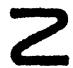
\includegraphics[keepaspectratio]{images/part002_a77d6c20.jpg}}

On the other hand, AB need not be closed when A is closed, even if B is closed too (cf.~§ 4, no. 1, Corollary 1 to Proposition 1).

* For example, in the additive group of the real line \(\mathbf{R}\) , the subgroup \(\mathbf{Z}\) of the rational integers is closed, and so is the subgroup \(\theta\mathbf{Z}\) consisting of all integer multiples \(n\theta\) of an irrational number \(\theta\) ; but the subgroup \(\mathbf{Z} + \theta\mathbf{Z}\) of \(\mathbf{R}\) , which is the set of all real numbers \(m + n\theta\) (where \(m\) and \(n\) take all integer values) is not closed in \(\mathbf{R}\) , as we shall see in Chapter V, § 1.

Again, let A be the subset of the additive group of \(\mathbf{R} \times \mathbf{R}\) which consists of all \((x, y)\) pairs such that \(x \geqslant 0\) and \(0 \leqslant y \leqslant 1 - \frac{1}{x + 1}\) ; and let B be the set of all pairs \((x,0)\) , as x runs through R. A and B are closed, but \(A + B\) is the set of all pairs \((x,y)\) such that \(0 \leqslant y < 1\) , and is not closed in \(R \times R\) .

Let X be a topological space and let f and g be two mappings of X into a topological group G. If f and g are continuous at a point \(x_{0}\) of X, then so are \(\overline{f}^{1}\) and \(fg\) (*), by Theorem 2 of Chapter I, § 2, no. 1. In particular, the continuous mappings of X into G form a subgroup of the group \(\mathbf{G}^{\mathbf{x}}\) of all mappings of X into G.

Again, let \(f\) and \(g\) be two mappings of a set \(\mathbf{X}\) , filtered by a filter \(\mathfrak{F}\) , into a Hausdorff topological group \(\mathbf{G}\) . If \(\lim_{\mathfrak{F}} f\) and \(\lim_{\mathfrak{F}} g\) exist, then so do \(\lim_{\mathfrak{F}} \overline{f}^1\) and \(\lim_{\mathfrak{F}} fg\) , and we have (Chapter I, § 7, no. 4, Proposition 9, Corollary 1)

\[
\lim _ {\mathfrak {F}} \overline {{f}} ^ {- 1} = (\lim _ {\mathfrak {F}} f) ^ {- 1},\tag{1}
\]

\[
\lim _ {\mathfrak {F}} f g = (\lim _ {\mathfrak {F}} f) (\lim _ {\mathfrak {F}} g).\tag{2}
\]

When G is a commutative group, written additively, the axiom (GT') indicates that \((x, y) \to x - y\) is a continuous mapping. If f and g are mappings of a topological space X into G, continuous at a point \(x_{0}\) , then f - g is continuous at this point. The formulas (1) and (2) can be transcribed similarly.
% semantic-fragments: legacy-input-seam
\relax{}
